\chapter{Related Work}
\label{chap:related}
In this section the related work will be presented.
For this, the related work is categorized into three categories:
\begin{itemize}
    \item \gls{AutoML} frameworks for classification
    \item Parameter optimization for clustering. 
    \item Meta learning for clustering
\end{itemize}

The related work for these categories will be shown in the following sections.

\section{AutoML Frameworks for classification}

In this section, two AutoML systems will be described in more detail.
These are Auto-Weka and Auto-sklearn.

\subsection{Auto-Weka}
\begin{itemize}
    \item Auto-Weka \cite{ThorntonAuto-WEKA:Algorithms, Kotthoff2017Auto-WEKAWEKA} was one of the first \gls{AutoML} systems.
    \item Used Bayesian Optimization to tackle the \gls{CASH} problem.
    \item Actually, \gls{BO} only for hyperparameter selection, but they used the algorithm as top-level parameter and depending on that value they selected the other hyperparameters.
    \item Basic architecture is shown in \cref{fig:autoweka}.
    Input for the system is budget, training data and a metric, according to which the optimizer is going to find the best model.
    As long as budget is left, the optimizer runs, which means the model is executed on the training data, then evaluated, stored and then the most important part, the next model is selected.
    \item Model has to be chosen in intelligent way, because limited budget and not able to search whole algorithm and their hyperparameter space.
    \item Optimizer there is Bayes Optimizer, more specifically they used \gls{SMAC} \cite{HutterSequentialConfiguration} and \gls{TPE} \cite{BergstraAlgorithmsOptimization}.
    \begin{figure}
        \centering
        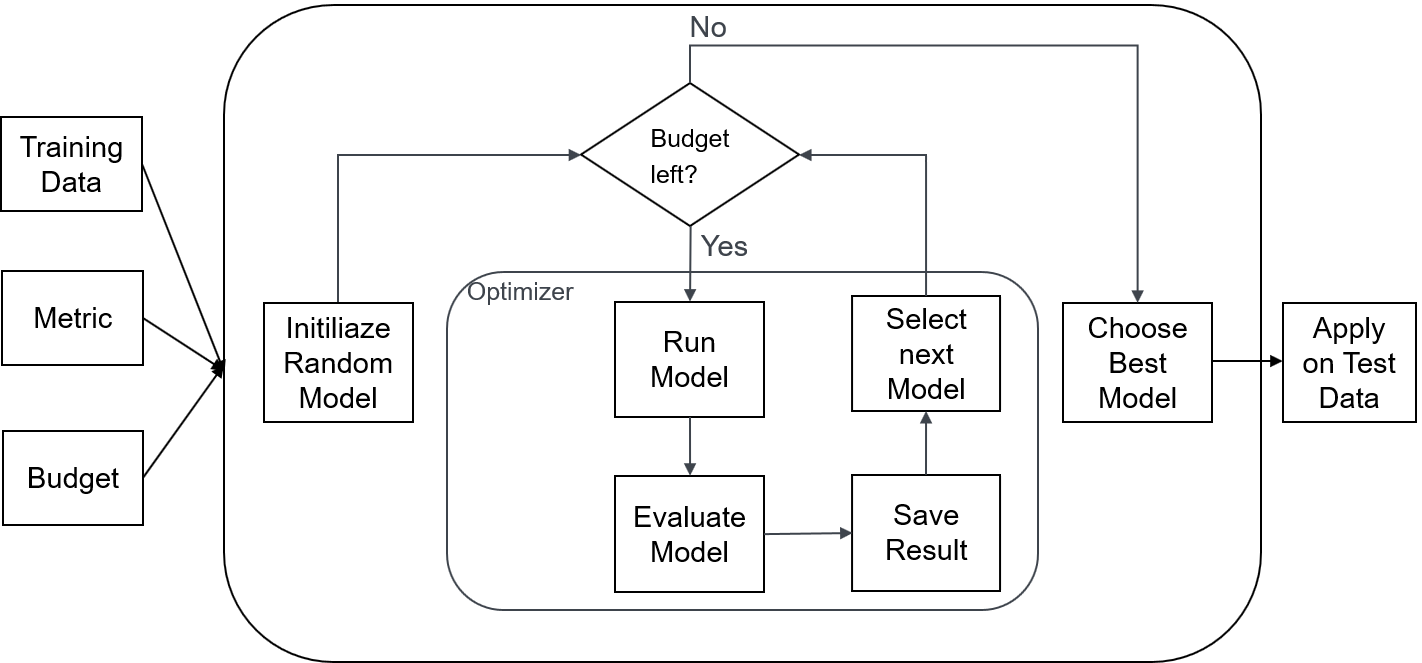
\includegraphics[width=0.7\textwidth]{graphics/auto_weka_arch.png}
        \caption{General architecture of the Auto-Weka system.}
        \label{fig:autoweka}
    \end{figure}
    \item Took all classifiers available in Auto-Weka. 
    They also used two ensemble classifiers and treated them as classifiers, but they only allowed five classifiers at maximum in the ensemble, such that the configuration space does not get too large.
    \item They were able to show that this approach is better than just running all algorithms with default hyperparameters and then choosing the best one (according to metric).
    \item They also showed that there approach performs in 11/21 cases with \gls{SMAC} and in 4/21 cases with \gls{TPE} regarding the test performance. Random Search in 2/21 and Grid Search in 4/21 cases.
\end{itemize}

\subsection{Auto-sklearn}
Auto-sklearn \cite{Feurer2015EfficientLearning} is based on the machine learning library scikit-learn \cite{PedregosaFABIANPEDREGOSA2011Scikit-learn:Perrot}.
They built the concept based on the Auto-Weka concept and extended it with two components.
\begin{itemize}
    \item General architecture of Auto-sklearn is shown in \cref{fig:autosklearn}.
    \begin{figure}
        \centering
        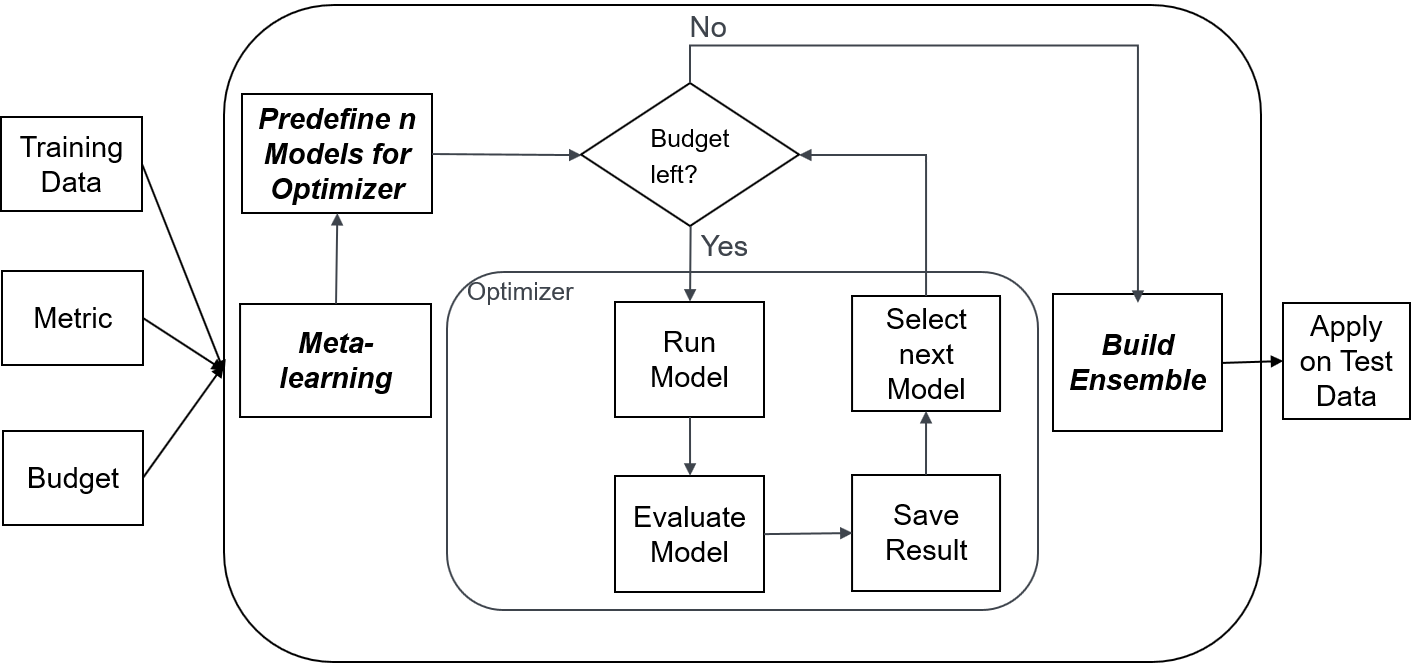
\includegraphics[width=0.7\textwidth]{graphics/auto_sklearn_arch.png}
        \caption{Basic architecture of Auto-sklearn. The components that are added compared to the Auto-Weka system (see \cref{fig:autoweka}) are marked as bold.}
        \label{fig:autosklearn}
    \end{figure}
    \item General same as Auto-Weka but \textit{meta-learning} and \textit{build ensemble} components are added.
    \item 
\end{itemize}

\iffalse

The basic architecture of their approach is shown in \Cref{fig:autosklearnArch}.
\begin{figure}
\centering
    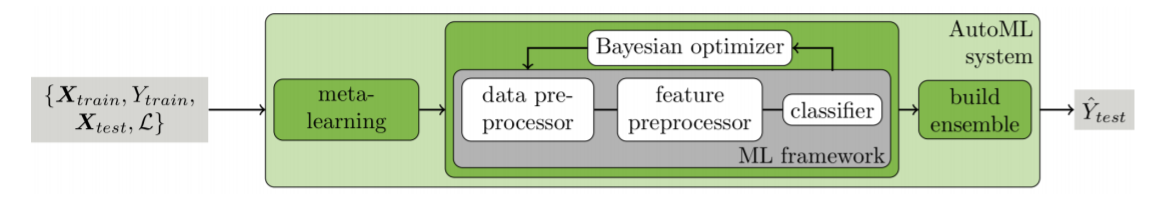
\includegraphics[width=\textwidth]{graphics/autosklearn_architecture.png}
    \caption{Basic workflow of the AUTO-SKLEARN system \cite{Feurer2015EfficientLearning}.}
    \label{fig:autosklearnArch}
\end{figure}
\fi

Meta-learning \cite{Brazdil2010MetalearningMining.} is a  method that learns from the performance of learning algorithms across datasets and applies it on new unseen datasets.
For this 38 meta-features, which represent the characteristics of a dataset, were extracted from the training datasets in an offline phase.
They also run SMAC \cite{HutterSequentialConfiguration} for 24 hours with 10-fold cross-validation on two-thirds of the data and the ML instance that had the best performance on the third one was stored.
In the online phase, for a new dataset, the meta-features were extracted and the datasets from the offline phase were ranked by the $L_1$ distance. 
The ML algorithms (that performed best in offline phase) of the 25 nearest datasets were then used and Bayesian optimization were run on them.
\iffalse
\begin{figure}
\centering
    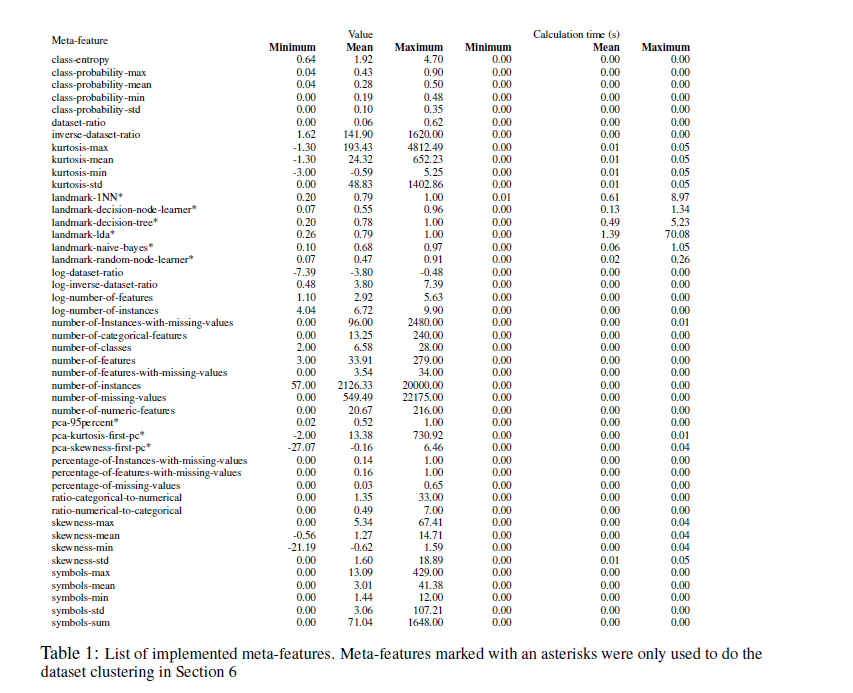
\includegraphics[width=\textwidth]{graphics/meta_features_autosklearn.png}
    \caption{Table of meta-features that were used in AUTO-SKLEARN \cite{Feurer2015EfficientLearning}.}
    \label{fig:MetaFeatureAutoSklearn}
\end{figure}
\fi

It has to be noted that the landmarking \cite{Pfahringer2000Meta-LearningAlgorithms} method was not used because of the computational complexity in the online phase, which makes it impractical in practice.

The second added component is the ensemble building component.
Instead of just taking the model that performs best, a number of models that also performed well are stored and to construct an ensemble out of them.
Because of this, the limit of just having one hyperparameter setting is lifted.
Building uniformly weighted ensemble of models found by \gls{BHO} did not work well.
Therefore ensemble selection \cite{CaruanaEnsembleModels} (which also performed better than stacking and gradient-free numerical optimization) was used.
Basically, it is a greedy procedure that starts with an empty ensemble and then iteratively adds a model that maximizes the validation performance.
\iffalse
The pseudocode is shown in \Cref{fig:ensemblePseudocode}.
\begin{figure}
\centering
    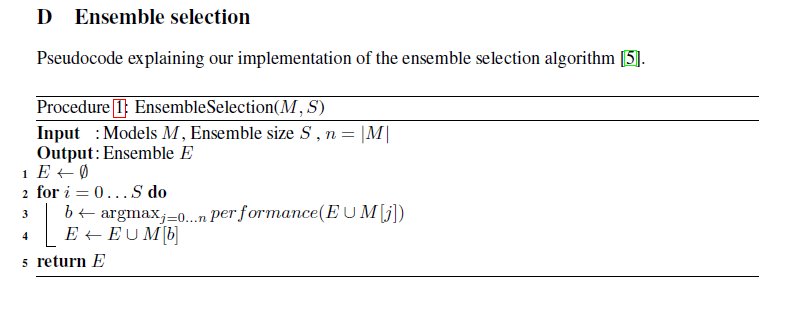
\includegraphics[width=\textwidth]{graphics/ensemble_selection_pseudocode.png}
    \caption{Pseudocode of the ensemble building algorithm \cite{Feurer2015EfficientLearning}.}
    \label{fig:ensemblePseudocode}
\end{figure}
\fi
Auto-sklearn only considered classification algorithms, so unsupervised learning methods like clustering were not taken into account.
But an important aspect of this work is to transfer the concepts of meta-learning and the used optimizers to clustering.

It has to be mentioned that there are a lot of more systems that have similar concepts, some examples are:

\begin{itemize}
    \item TPOT \cite{HomeTPOT}
    \item MLBox \cite{HomeDocumentation}
    \item H2O \cite{OverviewDocumentation}
    \item TransmogrifAI \cite{TransmogrifAIEngineering}
    \item Google Cloud AutoML \cite{CloudCloud}
    \item Microsoft Azure Automated ML \cite{AnnouncingAzure}
    \item More tools can be found in \cite{Elshawi2019AutomatedChallenges}
\end{itemize}
\xtodo{Short description for each tool? + fix reference}

\section{Meta-Learning for Clustering}

\xtodo{Overwork this. Just notes taken from the very very beginning.}

For clustering there are much less studies than for classification.

In \cite{DeSoutoRankingApproach} a meta-learning approach for ranking and selecting clustering algorithms was proposed.
They divided the architecture of their approach into three parts: \begin{inparaenum}
\item The feature extractor, which extracts the meta-features from a given dataset, 
\item the meta-learner, which applied  a regression algorithm on the extracted meta-features of the training data and applied to the validation data to generate a ranking of algorithms.
\item The database, which stores the training data with the extracted meta-features and also a ranking for this dataset for each algorithm.
\end{inparaenum}
In the first part, 8 meta-features were extracted which are mainly based on statistical
measures.
A list of this meta-features with description is given in \Cref{tab:8metafeatures}.
% Please add the following required packages to your document preamble:
% \usepackage{booktabs}
\begin{table}[]
\centering
\resizebox{\textwidth}{!}{%
\begin{tabular}{@{}ll@{}}
\toprule
Meta-feature & Description                                                                                                                                           \\ \midrule
LgE$_{10}$  & Describes the number of instances and takes it to the $log_{10}$, so LgE = $log_{10}(n)$.                                                             \\
LgREA        & Describes the log of ratio of the number of attributes by the number of instances. So LgREA = $log_{10} \frac{d}{n}$.                                 \\
PMV          & Percentage of missing data values.                                                                                                                    \\
MN           & Multivariate normality, which is the proportion of $T^2$ that are within 50 \% of the of a Chi-squared distribution.                   \\
SK           & Skewness of the $T^2$ vector.                                                                                                          \\
Chip         & Describes the type of microarray that was used (either cDNA or Affymetrix).                                                                           \\
PFA          & Percentage of attributes that were kept after the attribute selection filter.                                                                         \\
PO           & Percentage of outliers. These were measured by taking two times the $T^2$ \\
 & vector if it was two standard deviations away from the mean. \\ \bottomrule
\end{tabular}
}
\caption{List of meta-features that were used in \cite{DeSoutoRankingApproach}.}
\label{tab:8metafeatures}
\end{table}
In the second part, 7 clustering algorithms were considered: single linkage (SL), complete linkage (CL), average linkage (AL), K-means (KM), mixture model clustering (M), spectral clustering (SP) and Shared Nearest Neighbors.
The ranking was done by building a regressor for each clustering algorithm.
For this, datasets were used with the extracted meta-features.
The regression was done using the regression Support Vector Machines (rSVM) algorithm.
In the third part, the database, the dataset was stored with its meta-features and with the ranking for each algorithm. 
For each ranking, the result of an algorithm was compared to the gold-standard using the corrected Rand index \cite{Jain1988AlgorithmsData} (that index is only used for the evaluation).

The evaluation was done using 32 datasets from the micro-array domain.
They used leave-one-out crossfold for the validation, using each time 31 datasets for training and one for validation.
They assumed the ideal ranking is the ranking that was given by the corrected rand index.
Then the ranking that was generated from their meta-learner was compared to the ideal ranking by using the Spearman's rank correlation coefficient.
They showed that there approach could significantly are more correlated to the ideal ranking compared to the standard ranking.

Though they only used datasets from a very specific domain, the cancer gene expression microarray domain.
Also they did not consider the parameters at all, since they just used the "optimal" parameters.
Also they used only 8 metafeatures, where two of them can only be applied to their domain.
They also evaluated only one clustering measure, the corrected rand index, which is also an external validation measure.

In \cite{GomesFerrari2015ClusteringMethods} a similar concept for their meta-learning approach is used. 
One novelty in their approach was that they divided the set of meta-features for clustering in distance-based and attribute-based meta-features.
The distance-based meta-features were all meta-feature that can be calculated from the distance among each pair of instances in one dataset.
These include the mean, variance, standard deviation, skewness and kurtosis measures.
Also they examined how many percent of values are in a certain interval ($[0,~  0.1], ~  (0.1, ~ 0.2], \dots, ~ (0.9, ~ 1]$) and how many percent of values are in an absolute Z-score interval of $[0,~ 1),~ [1, ~ 2),~ [2, ~ 3)$ and $ [3, ~ \infty )$.
The attribute-based meta-features were meta-features that are based on the attributes of a dataset, so, e.g., the number of instances, attributes etc.
Overall 19 distance-based and 9 attribute-based meta-features were used.
They also used 7 clustering algorithms for algorithm recommendation.
For the ranking of the clustering algorithms they used different internal validation measures.
Therefore they created one ranking for each internal validation measure.
For example they used the Silhouette score and each clustering algorithm had a ranking for this measure based on the evaluated Silhouette score on the according dataset.
To combine the rankings from each of the ten internal validation measure they proposed to new methods: \begin{inparaenum}
\item The \textit{score} ranking, where each algorithm got points according to their ranking in the validation measure (e.g., 10 points for first rank, 8 for second and so on) and then the points were summed up for a new ranking.
\item The \textit{winner} ranking, where the number of victories for each validation measure was taken into account.
\end{inparaenum}
Given a new dataset, to determine which dataset is the "nearest" dataset in the meta-knowledge database, the k-Nearest-Neighbor classification algorithm was used on the meta-features.
For that purposed they also evaluated different values for the k in the kNN algorithm, ranging from 1 to 11.
There $k=5$ was used for the further experiments, because the deviation was not so high for this value.
For the evaluation also leave-one-out crossfold validation was used and to measure the performance of the recommended ranking according to the ideal ranking, Spearman's Rank Coefficient was used.
The experiments were performed on 84 datasets from the UCI repository.
They considered first only the distance-based meta-features, then the attribute-based and then hybrid based (using distance- and attribute-based meta-features) and combined all of them with every of the three ranking methods (average, score, winner).
The results showed that the best results were obtained for using the distance-based meta-features (regardlessly of the ranking method).
From the three ranking methods average, winner and score, the score ranking showed the best results.
Overall the novelty in this paper was to use the distance-based meta-features, using multiple internal indices and combine the different rankings for the algorithm by the score-ranking. 
Also they used more datasets than in the works before.
But in the evaluation the parameters for each clustering algorithm were fixed and it was not considered how to choose the best parameters or even how changing the parameters affect the results.
So they were no research done regarding hyperparameter optimization for clustering.
Also the authors state that more investigation should be done in finding more meta-features that can be extracted.

In \cite{Soares2009AnData} two meta-learners were used, the Multi-layer Perceptron (MLP) and the Support Vector Regressor (SVR).
They evaluated two sets of meta-features, which both contained 9 meta-features.
Both sets contained 4 meta-features regarding statistics about the dataset ($log_10$ of the number instances, attributes, the multivariate normality test and the percentage of outliers).
In $M_1$ the other five meta-features that contains univariate statistics (quartiles, skewness and kurtosis). 
In contrast, $M_2$ also conatains the four meta-features mentioned above and five that are based on the $T^2$ vector.
These contain three quartiles, skewness and the kurtosis of the $T^2$ vector.
For the algorithm selection, 9 clustering algorithms were taken into account and the ranking was done using a global error rate.
For the evaluation 160 arfticially generated datasets were used, which are based on an gaussian or an ellipsoid cluster generator.
The average Spearman's coefficient was used to compare the actual ranking to the ideal ranking.
The results showed that for both sets of meta-features and both meta-learners the results were more correlated to the ideal ranking than for the default ranking.

In \cite{NascimentoMiningData} meta-learning was used to derive knowledge from the training examples and to generate rules out of it, which automatically decide which clustering algorithm should be used.
For this seven clustering algorithms were used and they evaluated six meta-learning algorithms for: J48, PART, MLRules, Random Forest, k-NN and Support Vector Machine.
For the rule construction they used the MLRules algorithm and created 100 rules and selected the 10 best ones (highest weights) for the evaluation.
The evaluation was done on 36 different cancer data sets.
The extracted meta-features included the eight ones from \cite{DeSoutoRankingApproach} that can be seen in \cref{tab:8metafeatures} and extended them with 5 other meta-features. One was the normalized relative entropy (NRE), that is an indicator for the unifrom distribution of samples among classes. Then the  $SC_{10}$ and $SC_{15}$, which stand for ``small'' clusters and is a measure of number of classes with size inferior to the given thresholds 10 and 15.
They also included a similar measure for ``big'' clusters and at last the number of k-NN outliers were taken into account.

In \cite{Pimentel2019AMeta-learning} a new set of meta-features that combines correlation and dissimilarity is used, where the correlation measure is the main novelty of their approach.
In their work, 10 clustering algorithms were considered for the algorithm selection problem.
For assessing the quality of clustering results, 10 internal indices were used.
They also evaluated two meta-learners, namely the k-NN and random forests.
In the evaluation they compared their set of meta-features to other existing set of meta-features.
The experiments were performed on 219 datasets which were taken from OpenML from different domains, such as engineering, biology or physics.
Also they compared their algorithm selection system with existing ones.
The results showed that their approach performed better than the ones that are already existing in the literature when using k-NN as meta-learner.


In \cite{Corchado2019AConformations}, the authors try to estimate the number of clusters using meta-learning.
For this, they are using quality indices to describe the inner structure of the dataset.
They distinguished between two scenarios: Real-world and synthetic datasets.
The real-world datasets were categorized into binary and multi-class problems.
The aim was now to predict for a new dataset, if it is a binary or a multi-class dataset.
For the synthetic-datasets, the number of clusters ranged from 2 to 10 and in contrast to the real-world datasets, the aim was to estimate the concrete number of clusters.
The apprach was divided into three stages.
The first was the collection of meta information.´
So, how many meta-examples are used, the meta-features for each meta-example and the corresponding class label.
For the meta-features, 20 well-known inter cluster quality indices were used. 
For this, k-means was executed with for 9 different k's, ranging from $k=2$ to $k=10$, resulting in 180 meta-features that were extracted for each meta-example.
For the real-world the datasets the class label for each meta-example was either B (for binary) or MC (for multi-class).
For the synthetic datasets, the concrete number of clusters was the class label.
The second stage was the model building stage.
In this they first applied a one-class support vector machine (OCSVM) to determine if it is uniform data or not (so if they are even 2 or more clusters).
Then for those that have at least 2 or more clusters, a decision is built from the meta-features (so the qualitiy indices) using the C4.5 algorithm.
This helps to indicate which quality indices are most important (the ones on the top-level nodes and that are appearing most times).
The third stage was then the application stage, where the built model was applied to new unseen data.
For this, all 180 quality indices are computed for the new dataset and then passed to the C4.5 model, which then determined the cluster cardinality.
For the evaluation, 30 real-world datasets from the UCI repository were used, but for each of them 25 new datasets were generated using stratified sampling.
For the synthetic datasets, 2250 datasets were generated according to a cluster generator method \cite{QiuBrigham2006GenerationSeparation}.
Although the authors were able to address the problem with unsupervised data characterization predicting the number of clusters (or at least binary or not for real world datasets) using meta-learning, the effort for predicting a new unseen dataset is unacceptable high.
For a new unseen dataset, k-means has to be executed nine times (for $k=2, \cdots, 9$) and for each of this results, 20 quality indices have to be calculated. 
Also the authors did not tackle the problem of algorithm selection for clustering.

The existing literature for algorithm selection for clustering mostly use meta-learning to address this problem.
They all follow the same principle by storing meta-examples in some kind of database.
These contain meta-features together with some quality indices.
These indices are used to define an "ideal" ranking for the algorithms.
If more than one quality index is used then an aggregation of the different indices has to be defined to get one ranking for the algorithms.
When a new unseen dataset arrives, a meta-learner is used to predict the ideal algorithm for this dataset.
The most common used learners are either k-NN or random forests.
The approaches distinguish each other by different quality indices, different meta-features, different meta-learners, varying number of datasets that are used to build the meta-learning system and the number of clustering algorithms that are used.
Most of them also have in common that they do not take different parameter settings of the algorithm into account, but instead use a fixed parameter setting , which is most often the "optimal" setting if known in advance. 
The only exception here is \cite{Corchado2019AConformations} since they are trying to estimate the number of clusters using meta-learning.
But their approach is not feasible for real-world scenarios since 180 quality indices have to computed.
They also do not adress the algorithm selection problem.

\section{Hyperparameter Optimization for Clustering}

\begin{itemize}
    \item Usual process is to define search space and run clustering algorithm in this search space.
    \item Use some metric to evaluate the result.
    \item Then either choose best metric value (these are called relative metrics) or use elbow method.
    \item Also automated methods that do not require to define a search space or to run algorithm.
    \item Explain basic procedure of Xmeans \cite{Pelleg2000X-means:Clusters} /Gmeans \cite{HamerlyLearningK-means}.
    \item Basic procedure is to start with one cluster.
    \item Then split each cluster and if some criterion is met, then accept the split.
    Otherwise reject the split.
    \item Stop if no more splits were perfomred.
    \item Difference is in the criterion that can be met.
    \item Both algorithms implemented in PyClustering library \cite{NovikovPyClustering:Archive}.
    
\end{itemize}


Although the related work already investigated effort in using AutoML concepts for clustering, they still lack the following:

\begin{itemize}
    \item They did not use model-based hyperparameter optimization for clustering (like Bayesian Optimization as exmaple).
    \item There is no holistic taxonomy for the meta-features that can be used for clustering.
    \item Research was done in using algorithm selection with meta-learning or hyperparameter optimization for clustering, but it was not tried to combine both, so there is no system that considers algorithm selection and hyperparameter optimization together for clustering.
    \item Different evaluation methods were used for the ranking of the appropriate algorithms in the algorithm selection phase.
\end{itemize}